\documentclass[11pt]{article}
\title{Lenses}
\author{https://github.com/heptagons/lenses}
\date{2024/1/4}

\usepackage{graphicx}

\usepackage[margin=0.75in]{geometry}
\usepackage{float} % {figure}{H}
\usepackage{amsmath} % \dfrac

\def\mathbi#1{\textbf{\em #1}}

\begin{document}

\maketitle
\begin{abstract}
Lenses are equilateral hexagons resembling concave and convex optical lenses. Lenses consecutive six internal angles are $(\theta_1,\theta_2,\theta_3,\theta_1,\theta_2,\theta_3)$ where $\theta_1 = x\theta_0$, $\theta_2 = y\theta_0$, and $\theta_3 = z\theta_0$ where $\theta_0 = 2\pi/s$ is the base angle of symmetry $s = x + y + z$. Lenses can be formed adding and substracting rhombi or by intersecting equi-stars with others.
\end{abstract}

\section{Equi-stars}

\begin{figure}[H]
\centering
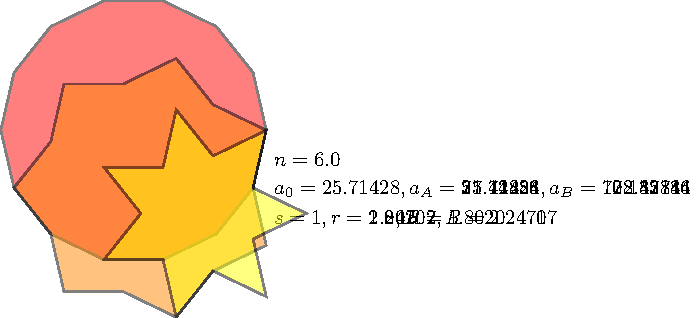
\includegraphics[scale=1]{stars/stars}
\caption{Equi-stars of symmetries $3$,$5$,$7$ and $9$.}
\label{fig:stars}
\end{figure}

Equi-stars are equilateral polygons with an even number of sides and vertices of at most two different angles. These stars can be defined with only two numbers: A symmetry integer $s$ and a minimum angle integer $a$ so the star is defined as $S(s,a)$. Here we are interested only in symmetries of the form $s=2n+1$ for $n=1,2,3...$. Every symmetry $s=2n+1$ has exactly $n$ different stars: $S(s,1),S(s,2),...,S(s,n)$. Stars of the form $S(s,n)$ correspond to the regular polygons of $2s$ sides.

Figure \ref{fig:stars} show the stars for the smaller symmetries in translucent colors and intersecting with others of the same symmetry. At $(i)$ we have for the symmetry $3$ the only star in red $S(3,1)$ which is the regular hexagon. At $(ii)$ we have for the symmetry $5$ the regular decagon in red $S(5,2)$ and the star $S(5,1)$ in yellow; the region in orange is the intersection of the two stars. At $(iii)$ for symmetry $7$ we have three stars: The equilateral 14-gon $S(7,3)$ in red, the $S(7,2)$ in yellow and the $S(7,1)$ in green. At $(iv)$ we have for the symmetry $9$ four stars: The regular 18-gon $S(9,4)$ in red, the $S(9,3)$ in yellow, the $S(9,2)$ in green and the $S(9,1)$ in blue.

\subsubsection{Lenses}

\begin{figure}[H]
\centering
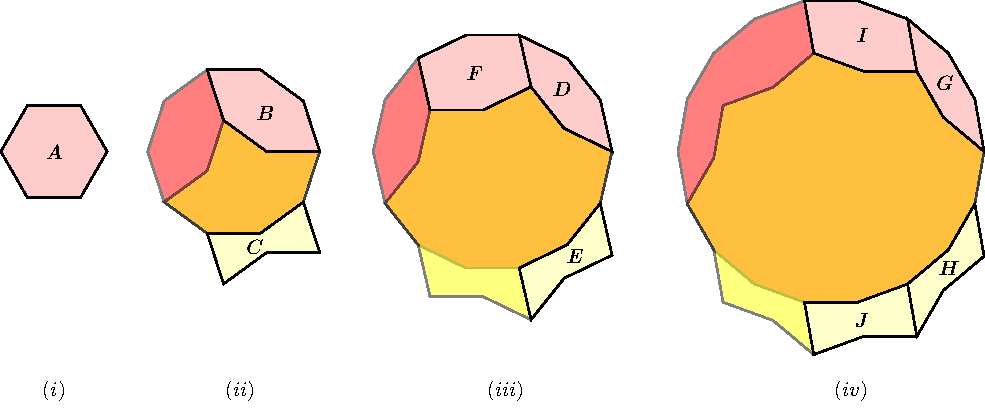
\includegraphics[scale=1]{stars/inter-1}
\caption{Lenses from equi-stars intersections symmetries $3$,$5$,$7$ and $9$.}
\label{fig:stars}
\end{figure}


\section{Symmetry $5$}

Symmetry $5$ is based in angle $\beta = \dfrac{2\pi}5$ and produces the two rhombi $(\mathbi{b},\mathbi{c})$ and the two lenses $(\mathbi{B},\mathbi{C})$.

\subsection{Rhombi (\mathbi{b},\mathbi{c})}

\begin{figure}[H]
\centering
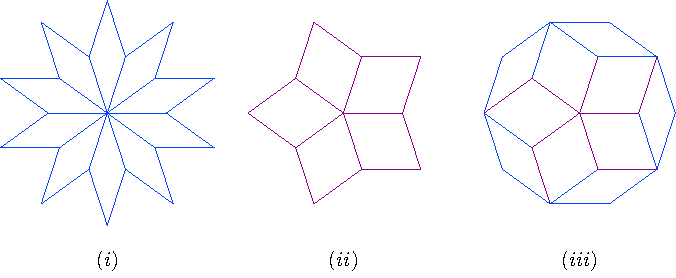
\includegraphics[scale=1.1]{bc/rhombi}
\caption{Rhombi $(\mathbi{b},\mathbi{c})$ from dissecting stars $S_{10}$.}
\label{fig:bc-rhombi}
\end{figure}

Figure \ref{fig:bc-rhombi} show the rhombi $(\mathbi{b},\mathbi{c})$. 
Inspecting the stars we get the areas simply adding their rhombi.
At $(i)$ the star $S_{10}(1,8)$ with area $A = 10\mathbi{b}$.
At $(ii)$ the star $S_{10}(2,6) = S_5(1,3)$ with area $A = 5\mathbi{c}$.
At $(iii)$ the regular decagon equivalvent to stars $S_{10}(4,4) = S_5(2,2)$ with area $A = 5\mathbi{b} + 5\mathbi{c}$. 
Table \ref {tbl:bc-angles} show the rhombi $(\mathbi{b},\mathbi{c})$ internal angles in terms of angle $\beta = 2\pi/5$ and areas for side equals to $1$. Dividing areas we find $\dfrac{\mathbi{c}}{\mathbi{b}} = 2\cos\left(\dfrac{\pi}5\right) = \dfrac{\sqrt5 + 1}2$.

\begin{table}[H]
\begin{center}
\begin{tabular}{|c|c c| l |}
\hline
Rhombus & $\theta_1$ & $\theta_2$ & Area \\ \hline\
$\mathbi{b}$ & $\beta/2$ & $4\beta/2$ & $\sin(2\beta) = \dfrac{\sqrt{10-2\sqrt5}}4 $
\\[1.2ex] \hline
$\mathbi{c}$ & $2\beta/2$ & $3\beta/2$ & 
$\sin(\beta) = \dfrac{\sqrt{10+2\sqrt5}}4 
= \mathbi{b}\cos\left(\dfrac{\pi}5\right) = \mathbi{b}\left(\dfrac{\sqrt5+1}2\right)$
\\[1.2ex] \hline
\end{tabular}
\caption{Rhombi $(\mathbi{b},\mathbi{c})$ internal angles and areas. $\theta_1 + \theta_2 = \pi$ and $\beta = 2\pi/5$.} 
\label{tbl:bc-angles}
\end{center}
\end{table}



\subsection{Regular pentagon and star $|5/2|$}

\begin{figure}[H]
\centering
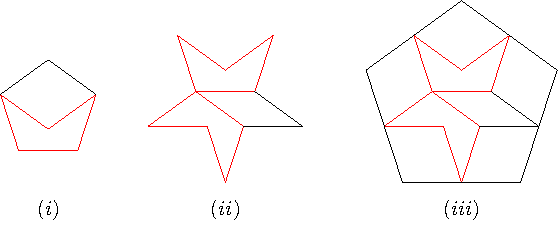
\includegraphics[scale=1.1]{bc/penta}
\caption{Regular pentagon $|5/1|$ at $(i)$. Star $|5/2|$ at $(ii)$. Double pentagon at $(iii)$.}
\label{fig:bc-penta}
\end{figure}

Figure \ref{fig:bc-penta} show regular pentagon and isotoxal star $|5/2|$ dissected with rhombi $(\mathbi{b},\mathbi{c})$ plus concave pentagons (in gray). Let $\mathbi{x}$ be the area of such gray piece. By inspection the area of regular pentagon at $(i)$ is $A_1 = \mathbi{c} + \mathbi{x}$ and the area of regular pentagon at $(iii)$ is $P_2 = \mathbi{b} + 5\mathbi{c} + 2\mathbi{x}$. Since the side of $A_2$ is the double of $A_1$ its area is four times so we can get the value of $\mathbi{x}$ in terms of $(\mathbi{b},\mathbi{c})$
\begin{align}
4P_1 &= P_4 \nonumber\\
4(\mathbi{c} + x) &= \mathbi{b} + 5\mathbi{c} + 2x\nonumber\\
x &= \frac{\mathbi{b} + \mathbi{c}}2
\end{align}

We use the value of $\mathbi{x}$ to get the areas of pentagon $(i)$ and star $(ii)$:
\begin{align}
A|5/1| &= \mathbi{c} + \mathbi{x} \nonumber\\
 &= \frac{\mathbi{b} + 3\mathbi{c}}2 \\
A|5/2| &= \mathbi{b} + 2\mathbi{x} \nonumber\\
 &= 2\mathbi{b} + \mathbi{c}
\end{align}

\subsection{Lenses (\mathbi{B},\mathbi{C})}

\begin{figure}[H]
\centering
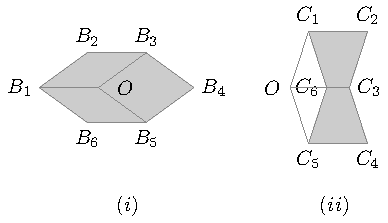
\includegraphics[scale=1.1]{bc/bc}
\caption{Lenses (\mathbi{B}, \mathbi{C}) build with rhombi (\mathbi{b}, \mathbi{c}).}
\label{fig:bc-lenses}
\end{figure}

Figure \ref{fig:bc-lenses} show lenses $(\mathbi{B},\mathbi{C})$ construction and two stars formed with them.
At $(i)$ we form the lense $\mathbi{B}$ with perimeter $\overline{B_1...B_6}$ adding two rhombi $\mathbi{b}$ ($\overline{B_1B_2B_3O}$ and $\overline{B_1OB_5B_6}$) and adding one rhombus $\mathbi{c}$ ($\overline{OB_3B_4B_5}$) so its area is $2\mathbi{b} + \mathbi{c}$. Lense $\mathbi{B}$ is equivalent to the hexagon $H_5(1,2,2)$.
At $(ii)$ we form the lense $\mathbi{C}$ with perimeter $\overline{C_1...C_6}$ adding two rhombi $\mathbi{c}$ ($\overline{OC_1C_2C3}$ and $\overline{OC_3C_4C_5}$) and substracting one rhombus $\mathbi{b}$ ($\overline{OC_1C_6C_5}$) so its area is $2\mathbi{c} - \mathbi{b}$. Lense $\mathbi{C}$ is equivalent to the hexagon $H_5(1,1,3)$.
Table \ref{tbl:bc-lenses-angles} show the lenses $(\mathbi{B},\mathbi{C})$ internal angles and areas.

\begin{table}[H]
\begin{center}
\begin{tabular}{|c|c c c| c |} \hline
Lense & $\theta_1$ & $\theta_2$ & $\theta_3$ & Area \\ \hline
$\mathbi{B}$ & $\beta$ & $2\beta$ & $2\beta$ & $2\mathbi{b} + \mathbi{c}$
\\[0.5ex] \hline
$\mathbi{C}$ & $\beta$ & $\beta$ & $3\beta$ & $- \mathbi{b} + 2\mathbi{c}$
\\[0.5ex] \hline
\end{tabular}
\caption{Lenses $(\mathbi{B},\mathbi{C})$ internal angles and areas in terms of rhombi $(\mathbi{b},\mathbi{c})$. $\theta_1+\theta_2+\theta_3 = 2\pi$ where $\beta = 2\pi/5$.} 
\label{tbl:bc-lenses-angles}
\end{center}
\end{table}



\begin{figure}[H]
\centering
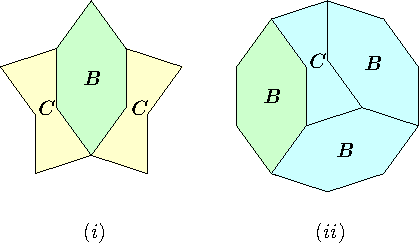
\includegraphics[scale=1.1]{bc/bc-stars-2}
\caption{Two stars dissected with lenses (\mathbi{B}, \mathbi{C}).}
\label{fig:bc-stars-2}
\end{figure}

Figure \ref{fig:bc-stars-2} show two stars dissected with lenses (\mathbi{B}, \mathbi{C}).
At $(i)$ the star $S_5(1,3)$ dissection implies its area is $A = \mathbi{B} + 2\mathbi{C} = 5\mathbi{c}$.
At $(ii)$ the regular decagon or star $S_5(2,2)$ dissection implies its area is $A = 3\mathbi{B} + \mathbi{C} = 5(\mathbi{b} + \mathbi{c})$.


% 7

\section{Symmetry $7$}

Symmetry $7$ is based in angle $\gamma = \dfrac{2\pi}7$ and produces the three rhombi $(\mathbi{d},\mathbi{f},\mathbi{e})$ and the three lenses $(\mathbi{D},\mathbi{E},\mathbi{F})$.

\subsection{Rhombi $(\mathbi{d},\mathbi{e},\mathbi{f})$}

\begin{figure}[H]
\centering
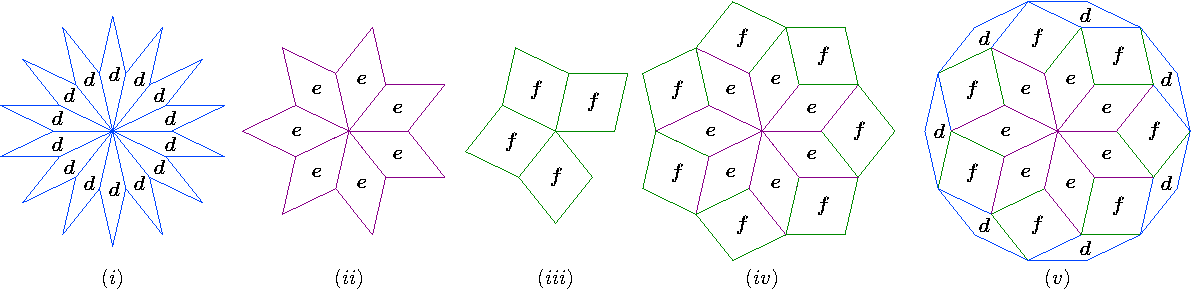
\includegraphics[scale=1]{def/rhombi}
\caption{Rhombi $(\mathbi{d},\mathbi{e},\mathbi{f})$ from dissected stars $S_{14}$. }
\label{fig:def-rhombi}
\end{figure}

Figure \ref{fig:def-rhombi} show rhombi $(\mathbi{d},\mathbi{e},\mathbi{f})$. 
Inspecting the stars we get the areas simply adding their rhombi.
At $(i)$ the star $S_{14}(1,12)$ with area $A = 14\mathbi{d}$. 
At $(ii)$ the star $S_{14}(2,10) = S_7(1,5)$ with area $A = 7\mathbi{e}$.
At $(iii)$ the star $S_{14}(4,8) = S_7(2,4)$ with area $A = 7(\mathbi{e} + \mathbi{f})$.
At $(iv)$ the regular 14-gon equivalent to stars $S_{14}(6,6) = S_7(3,3)$ with area $A = 7(\mathbi{d} + \mathbi{e} + \mathbi{f})$.
Table \ref{tbl:def-angles} show the symmetry 7 lenses internal angles based in angle $\gamma = 2\pi/7$ and the areas.

\begin{table}[H]
\begin{center}
\begin{tabular}{|c|c c| c |} \hline
Rhombus & $\theta_1$ & $\theta_2$ & Area \\ \hline\
$\mathbi{d}$ & $\gamma/2$ & $6\gamma/2$ & $\sin(3\gamma)$
\\[0.5ex] \hline
$\mathbi{e}$ & $2\gamma/2$ & $5\gamma/2$ & $\sin(\gamma)$
\\[0.5ex] \hline
$\mathbi{f}$ & $3\gamma/2$ & $4\gamma/2$ & $\sin(2\gamma)$
\\[0.5ex] \hline
\end{tabular}
\caption{Rhombi $(\mathbi{d},\mathbi{e},\mathbi{f})$ internal angles. $\theta_1 + \theta_2 = \pi$ and $\gamma = 2\pi/7$.} 
\label{tbl:def-angles}
\end{center}
\end{table}



\subsection{Regular heptagon and stars $|7/3|$ and $|7/2|$}

\begin{figure}[H]
\centering
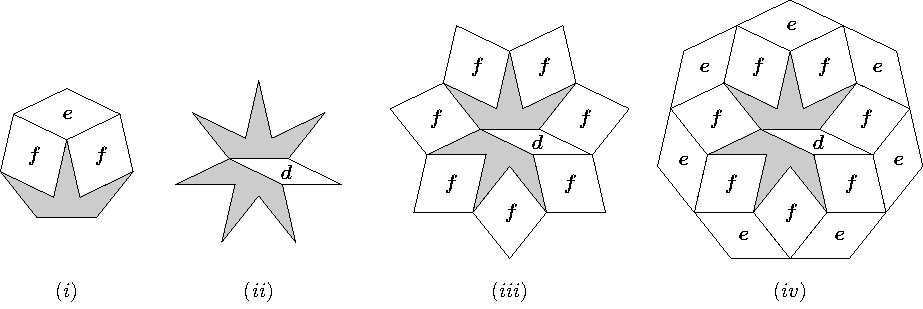
\includegraphics[scale=1.1]{def/hepta}
\caption{Heptagon $|7/1|$ at $(i)$. Star $|7/3|$ at $(ii)$. Star $|7/2|$ at $(iii)$. Double heptagon at $(iv)$.}
\label{fig:def-hepta}
\end{figure}

Figure \ref{fig:def-hepta} show regular heptagon and heptagrams dissected with rhombi $(\mathbi{c},\mathbi{d},\mathbi{e})$ plus equilateral concave heptagons (in gray). Let $\mathbi{y}$ be the area of such gray piece. By inspection the area of regular heptagon at $(i)$ is $A_1 = \mathbi{e} + 2\mathbi{f} + \mathbi{y}$ while the area of regular heptagon at $(iv)$ is $A_2 = \mathbi{d} + 7(\mathbi{e}+\mathbi{f}) + 2\mathbi{y}$. Since the side of $A_2$ is the double of $A_1$ its area is four times so we can get the value of $\mathbi{y}$ in terms of $(\mathbi{d},\mathbi{e},\mathbi{f})$:
\begin{align}
4A_1 &= A_2 \nonumber\\
4(\mathbi{e} + 2\mathbi{f} + \mathbi{y}) &= \mathbi{d} + 7(\mathbi{e}+\mathbi{f}) + 2\mathbi{y} \nonumber\\
\mathbi{y} &= \frac{\mathbi{d} + 3\mathbi{e} - \mathbi{f}}2
\end{align}

We use the value of $\mathbi{y}$ to calculate the areas of heptagon $(i)$ and stars $(ii)$ and $(iii)$ in terms of $(\mathbi{d},\mathbi{e},\mathbi{f})$:
\begin{align}
A|7/1| &= \mathbi{e} + 2\mathbi{f} + \mathbi{y} \nonumber\\
    &= \frac{\mathbi{d} + 5\mathbi{e} + 3\mathbi{f}}2 \\
A|7/3| &= \mathbi{d} + 2\mathbi{y} \nonumber\\
 &= 2\mathbi{d} + 3\mathbi{e} - \mathbi{f} \\
A|7/2| &= A\{7/3\} + 7\mathbi{f} \nonumber\\
 &= 2\mathbi{d} + 3\mathbi{e} + 6\mathbi{f}
\end{align}

\subsection{Lenses (\mathbi{D},\mathbi{E},\mathbi{F})}

\begin{figure}[H]
\centering
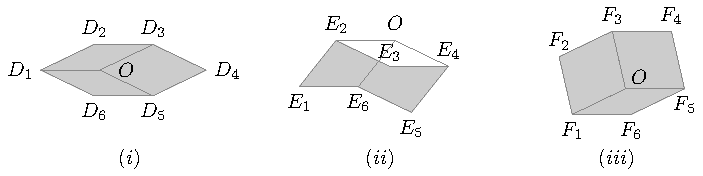
\includegraphics[scale=1.1]{def/def}
\caption{Lenses (\mathbi{D},\mathbi{E},\mathbi{F}) build from rhombi (\mathbi{d},\mathbi{e},\mathbi{f}).}
\label{fig:def-hexagons}
\end{figure}



Figure \ref{fig:def-hexagons} show lenses $(\mathbi{B},\mathbi{C})$ construction.
At $(i)$ we form the lense $\mathbi{D}$ with perimeter $\overline{D_1...D_6}$ adding two rhombi $\mathbi{d}$ ($\overline{D_1D_2D_3O}$ and $\overline{D_1OD_5D_6}$) and adding one rhombus $\mathbi{e}$ ($\overline{OD_3D_4D_5}$) so its area is $2\mathbi{d} + \mathbi{e}$. Lense $\mathbi{D}$ is equivalent to the hexagon $H_7(1,3,3)$.

At $(ii)$ we form the lense $\mathbi{E}$ with perimeter $\overline{E_1...E_6}$ adding one rhombus $\mathbi{e}$ ($\overline{E_1E_2OE_6}$) adding one rhombus $\mathbi{f}$ ($\overline{OE_4E_5E_6}$) and substracting one rhombus $\mathbi{d}$ ($\overline{E_2OE_4E_3}$) so its area is $-\mathbi{d} + \mathbi{e} + \mathbi{f}$. Lense $\mathbi{E}$ is equivalent to the hexagon $H_7(1,2,4)$.

At $(iii)$ we form the lense $\mathbi{F}$ with perimeter $\overline{F_1...F_6}$ adding two rhombi $\mathbi{f}$ ($\overline{F_1F_2F_3O}$ and $\overline{F_3F_4F_5O}$) and adding one rhombus $\mathbi{d}$ ($\overline{F_1OF_5F_6}$) so its area is $\mathbi{d} + 2\mathbi{f}$. Lense $\mathbi{F}$ is equivalent to the hexagon $H_7(2,2,3)$.
Table \ref{tbl:def-lenses-angles} show the lenses $(\mathbi{D},\mathbi{E},\mathbi{F})$ internal angles and areas.

\begin{table}[H]
\begin{center}
\begin{tabular}{|c|c c c| c |} \hline
Lense & $\theta_1$ & $\theta_2$ & $\theta_3$ & Area \\ \hline\
$\mathbi{D}$ & $\gamma$  & $3\gamma$ & $3\gamma$ & $2\mathbi{d} + \mathbi{e}$
\\[0.5ex] \hline
$\mathbi{E}$ & $\gamma$  & $2\gamma$ & $4\gamma$ & $-\mathbi{d} + \mathbi{e} + \mathbi{f}$
\\[0.5ex] \hline
$\mathbi{F}$ & $2\gamma$ & $2\gamma$ & $3\gamma$ & $-\mathbi{d} + 2\mathbi{f}$ 
\\[0.5ex] \hline
\end{tabular}
\caption{Lenses $(\mathbi{D},\mathbi{E},\mathbi{F})$ internal angles and areas in terms of rhombi $(\mathbi{d},\mathbi{e},\mathbi{f})$. $\theta_1+\theta_2+\theta_3 = 2\pi$ and $\gamma = 2\pi/7$.} 
\label{tbl:def-lenses-angles}
\end{center}
\end{table}



\begin{figure}[H]
\centering
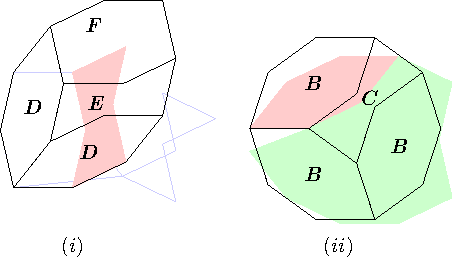
\includegraphics[scale=1.1]{def/def-stars-2}
\caption{Stars dissected with only lenses (\mathbi{D},\mathbi{E},\mathbi{F}).}
\label{fig:def-stars-2}
\end{figure}

Figure \ref{fig:def-stars-2} show stars $S_7(2,4)$ and $S_7(3,3)$ dissected with lenses (\mathbi{D},\mathbi{E},\mathbi{F}).
At $(i)$ we have star $S_7(2,4)$ and by inspection we deduce its area is $A = 2\mathbi{D} + 5\mathbi{E} + \mathbi{F}$. At $(ii)$ we have regular 14-gon (or star $S_7(3,3)$) and by inspection we deduce its area is $4\mathbi{D} + 3\mathbi{E} + 2\mathbi{F}$. Both stars have in common an area in green resembling a tree leaf. The star at $(i)$ also contains two regions in yellow resembling crowns while the star at $(ii)$ contains a region in cyan resembling a moon phase.

\begin{figure}[H]
\centering
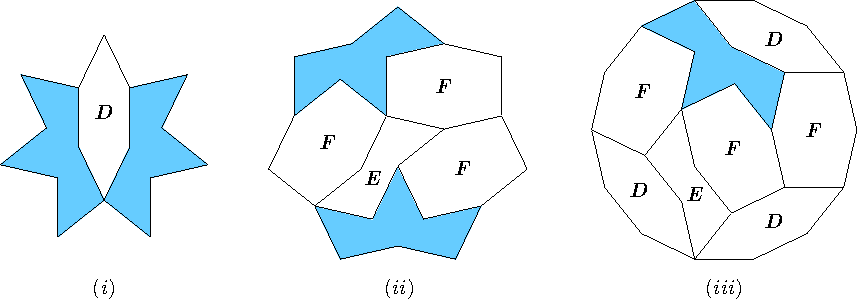
\includegraphics[scale=1.1]{def/def-stars-3}
\caption{Stars dissected with octagons \mathbi{$O_7$} (in blue) and lenses (\mathbi{D},\mathbi{E},\mathbi{F}).}
\label{fig:def-stars-3}
\end{figure}
 
Figure \ref{fig:def-stars-3} show Stars $S_7(1,5)$, $S_7(2,4)$ and $S_7(3,3)$ dissected with octagons \mathbi{$O_7$} (in blue) and lenses (\mathbi{D},\mathbi{E},\mathbi{F}). At $(i)$ we have the star $S_7(1,5)$ and by inspection we deduce its area is $A = \mathbi{D} + 2\mathbi{$O_7$}$. At $(ii)$ we have the star $S_7(2,4)$ and we can conclude its area is $\mathbi{E} + 3\mathbi{F} + 2\mathbi{$O_7$}$. Similarly the area of the 14-gon at $(iii)$ is $3\mathbi{D} + \mathbi{E} + 3\mathbi{F} + \mathbi{$O_7$}$. Comparing the areas of the two 14-gons of figures \ref{fig:def-stars-2} and \ref{fig:def-stars-3} we can find the area of \mathbi{$O_7$} in terms of $(\mathbi{E},\mathbi{F},\mathbi{G})$:
\begin{align}
4\mathbi{D} + 3\mathbi{E} + 2\mathbi{F} &= 
 3\mathbi{D} + \mathbi{E} + 3\mathbi{F} + \mathbi{$O_7$}\nonumber\\
\mathbi{$O_7$} &= \mathbi{D} + 2\mathbi{E} - \mathbi{F}
\end{align}

So we can calculate the area of star $S_7(1,5)$ in terms of $(\mathbi{E},\mathbi{F},\mathbi{G})$:
\begin{align}
S_7(1,5) &= \mathbi{D} + 2(\mathbi{D} + 2\mathbi{E} - \mathbi{F}) \nonumber\\
 &= 3\mathbi{D} + 4\mathbi{E} - 2\mathbi{F}
\end{align}


\end{document}
